
This chapter examines the capabilities of the intrusion detection techniques and algorithms presented earlier in the context of attacks on OAuth protocol flows, by developing a complete experiment environment, including the generation of a dataset and the implementation of an unsupervised anomaly intrusion detection approach.

Initially, Section \ref{sec:exp_setup} describes generally the process of the creation of the experimental environment for dataset generation and the involved systems that were implemented.

Section \ref{sec:impl_analysis} continues with describing the implementation of the data analysis algorithms utilized in this work, as well as the performance metrics applied to generate the results.

Finally Section \ref{sec:exp_results} presents and discusses the results of the implemented intrusion detection approach on the generated dataset.


\section{Implementation of the data generation environment}
\label{sec:exp_setup}

An essential piece for this research and its experiments is a complete testing environment for OAuth as at the time of this writing a dataset of network logs with specific attacks on OAuth does not exist. To generate a dataset to analyze it, an experimental environment was implemented containing multiple components as illustrated in figure \ref{fig:experimental_setup}. It consists of three main parts, the first part being the main OAuth services, which are the authorization server, the resource server, and the client, to make OAuth network traffic in general possible. The second part is the dataset generation part, which is done through fuzzing requests in the OAuth environment, which produces logs in the form of \emph{.pcap}-files through the logger services. The third and last part is the analysis part, which is initialized through the preprocessing of zeek, which produces several log files from which the created \emph{http.log}-files are getting processed in the analyzer component. The analyzer component executes the implemented algorithms to detect anomalies. It consists of an encoding step, where some textual data of the \emph{http.log} file get converted to a numerical representation using word embeddings, followed by clustering algorithms that try to detect anomalies in the encoded data.

\begin{figure}[H]
	\sffamily\footnotesize
	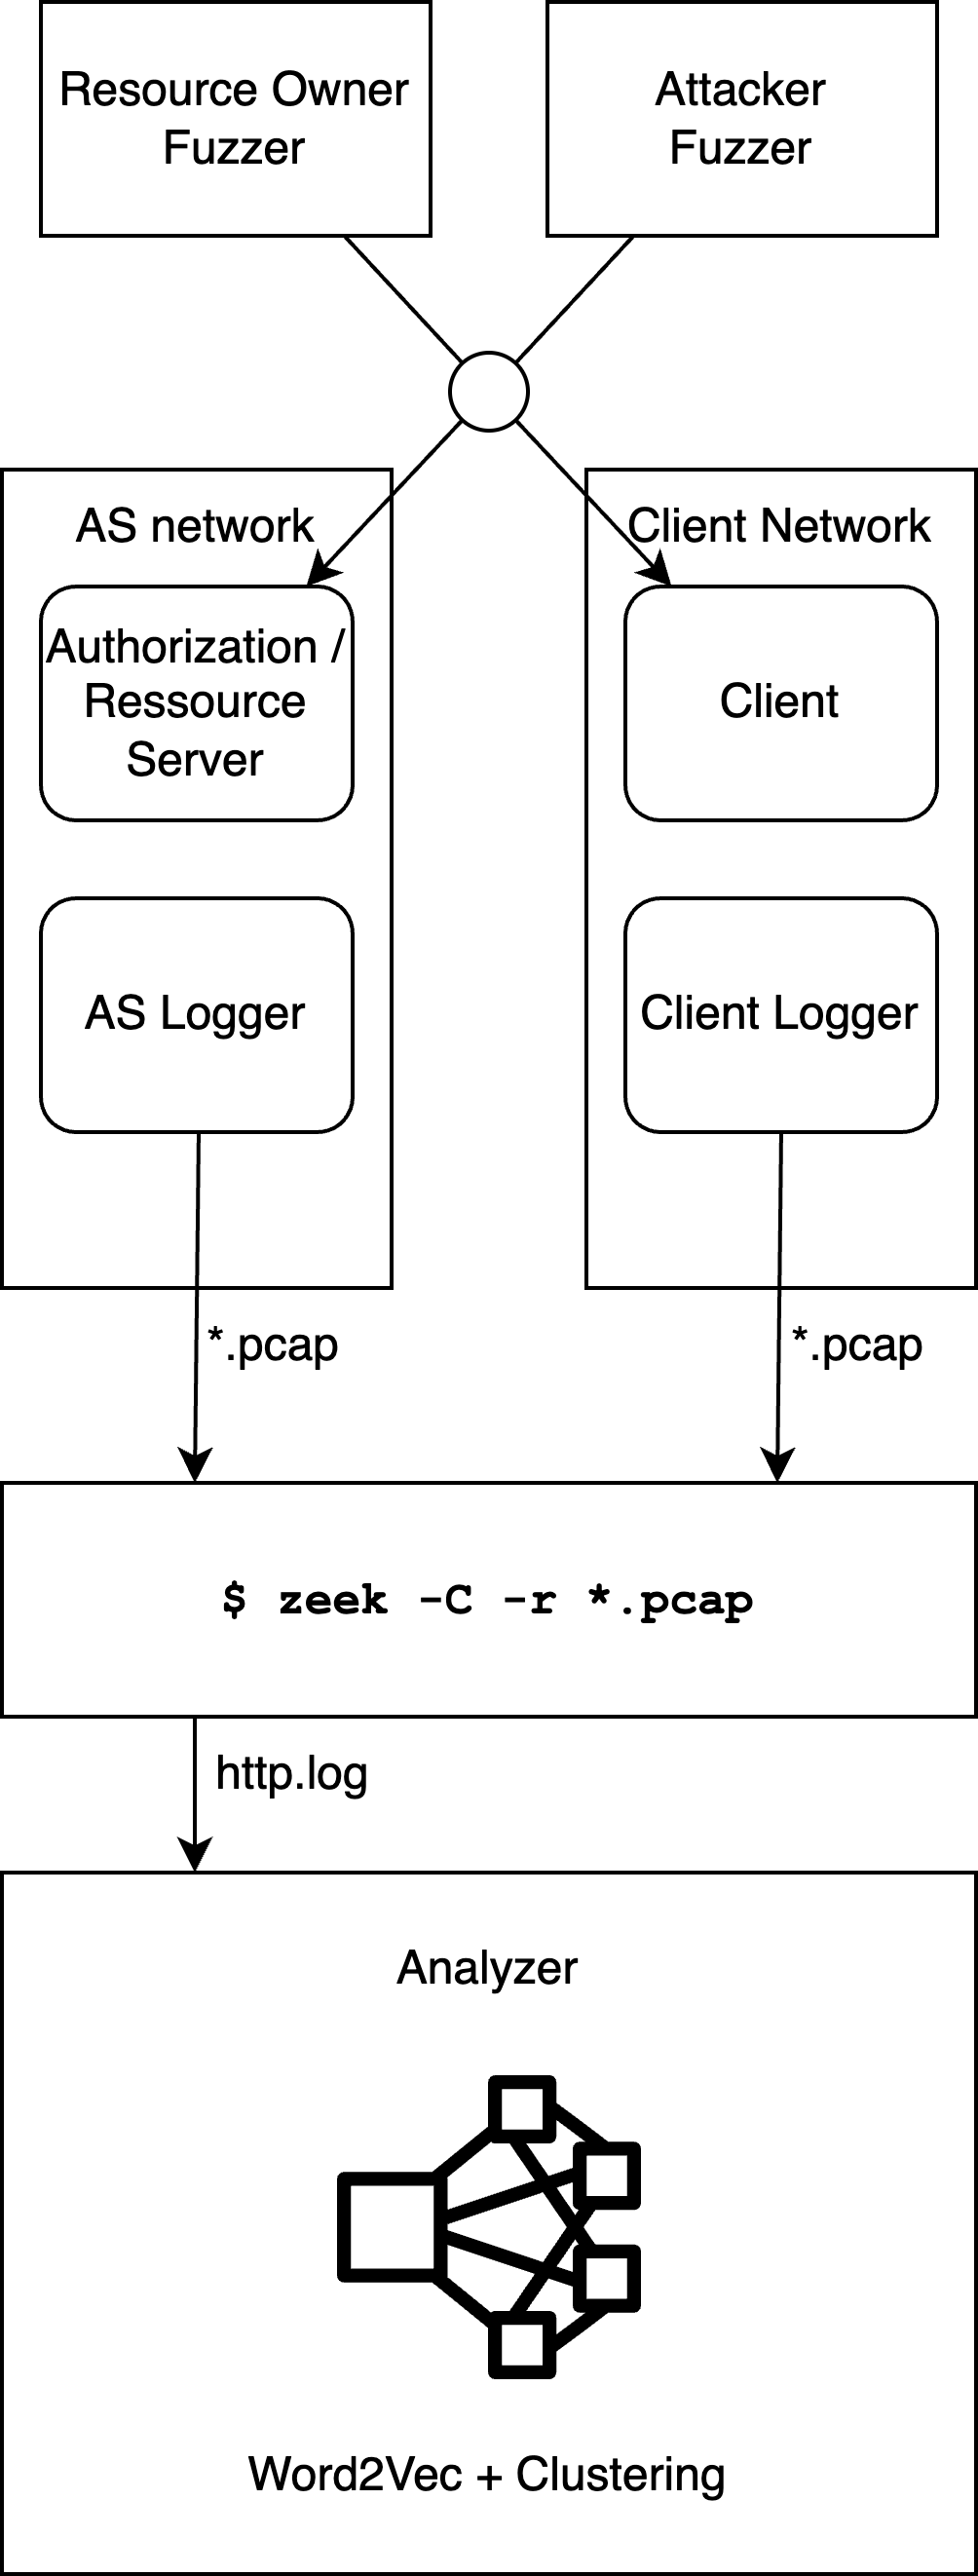
\includegraphics[width=0.5\textwidth]{pic/experimental_setup.png}
	\unitlength=0.75mm
	\special{em:linewidth 0.4pt}
	\linethickness{0.4pt}
	\caption{Overview of the environment for the experiments}
	\label{fig:experimental_setup}
\end{figure}

\subsection{OAuth setup}
For this first part, an OAuth environment was implemented, which consists of several subsystems that are needed to execute the OAuth protocol flow. It consists of two independent networks. The first network contains the authorization provider, resource server and a logging service, and the second network contains the OAuth client service and a logging service. The loggers produce \emph{.pcap}-files of all activity in their network using the popular tool \emph{tcpdump}, which is already available in most UNIX-based operating systems. The OAuth authorization framework is mostly modular. Therefore, the network logs are divided between the authorization server and the client, as in practice, mostly two different parties run these services. 

\subsubsection{Authorization Server and Resource Server}
The implementation of the authorization server and resource server is forked from the \emph{authlib} project version 1.2.1 \cite{authlib2023}. More specifically the \emph{Flask OAuth Providers} component is utilized for the authorization and resource server. To make the authorization process more vulnerable the mandatory PKCE feature was deactivated. Having the possibility to make adjustments like this, was the reason for forking the project, instead of importing it as a library. The authorization server implementation of \emph{authlib} offers four OAuth grants out of the box, which are among the most essential grants, namely \emph{implicit grant}, \emph{authorization code grant}, \emph{client credentials grant}, and \emph{resource owner password credentials Grant}. It also implements the \emph{PKCE} extension. Besides the authorization capabilities, the \emph{authlib} implementation also offers a protected resource in the form of an API, which is only accessible by authorized clients. The protected endpoint it offers returns the username of the currently authorized user. This API was extended with several endpoints allowing for the simulation of usual user-specific network traffic. Integrating the \emph{authlib} library into the experiment environment allows for the execution of valid OAuth protocol interactions, the simulation of usual network traffic, as well as the execution of attacks tampering with the redirection flow.

\subsubsection{Client application}
The client application as an additional component for the experimental setup is a simple static webpage that handles the authorization code grant. It can be used to generate traffic manually, but its primary purpose is to handle redirections as part of the different flows. It is written in HTML, CSS, and Javascript to utilize the Fetch API and the Browser Storage API. An implementation of redirect handling is shown in figure \ref{lst:redirect_handler}. The client is checking if the code query parameter is present in the currently active URL (line 6) when the page loads. If it is present it extracts it and retrieves an access token from the authorization server.

\begin{minipage}\linewidth
\begin{lstlisting}[language={java}, caption={Example implementation of authorization code handling at the client}, label={lst:redirect_handler}]
// fetch access token on page load, if the code query param is present
window.onload = function() {
	const params = new URLSearchParams(window.location.search);
	const client_id = "<pre-configured client ID>"

	if (params.has("code")) {
		const form = new FormData();
		form.append('grant_type', 'authorization_code');
		form.append('scope', '<some scope>');
		form.append('code', params.get("code"));
		form.append('client_id', client_id);
		fetch('<token endpoint of authorization server>', {
			method: 'POST',
			body: form
		})
	}
}
\end{lstlisting}
\end{minipage}

\subsection{Network setup and logging}
All services are hosted using containers in a docker environment. Technically these services are part of the same network at the docker host they are run on, but the logging services build overlay networks on the services they are observing. As visualized in figure \ref{fig:experimental_setup} there exist two logging services, one for the authorization and resource server and one for the client network. When the experiment environment is active, the logging services stream all network events to a \emph{.pcap}- file, which is accessible at the docker host through a volume. All communication is executed without TLS to be able to analyze all packets. In a real-world scenario this would not be the case, but mechanisms like internal proxies, who are acting as man-in-the middle would be able to inspect the network traffic unencrypted in that case as well.

\begin{minipage}\linewidth
\begin{lstlisting}[language={bash}, caption={Logger process}, label={lst:logging_service}] 
$ ethtool -K eth0 rx off tx off tso off;tcpdump -i eth0 -w /log/"$filename_prefix"-log-$(date +"%Y%m%d_%H-%M-%S").pcap
\end{lstlisting}
\end{minipage}

\subsection{Attacks}
\label{subsec:attacks}
For the attacks on OAuth several pre-conditions were established to make the OAuth environment vulnerable. PKCE as mentioned earlier has been made optional. There is not any CSRF protection in place, utilizing the state parameter. This leads to the attacks being harder to detect as omitting these parameters as an attacker, will not make a difference anymore compared to the usual traffic. Another assumption is that an attacker is at all times able to circumvent any whitelist for redirect URIs. This is simulated by allowing the URI of the attacker server in the securely implemented whitelist of \emph{authlib}. In addition, it is assumed that an attacker, who crafts a malicious link can make the victim use the malicious link, through phishing or similar techniques. Another precondition is that the victim is logged in at all times and if it is not logged in it will immediately complete the login process. To facilitate the attacks an attacker callback server has been implemented as well. Also, every HTTP request involved in an attack, especially the ones where the victim is visiting a maliciously crafted URL is labeled with a special header \emph{X-Is-Attack} with the name of the attack as its value, which is used for evaluating the detection success rate later, but omitted for the detection itself.

\subsubsection{Attacker callback server}
The attacker callback server is a service implemented using the Python \emph{http.server} library, which serves the purpose of a callback handler for attacks that redirect the victim's OAuth flows to the attacker. This means if an authorization code or access token ends up being redirected to this callback server it immediately completes OAuth flows with the stolen authorization codes or access tokens and generates traffic at the authorization server like this. An example implementation for such a callback handler is shown in figure \ref{lst:attacker_server}. The \emph{do\_GET} method (line 2) is executed, whenever a GET request reaches the attacker server. If this request contains an authorization code parameter (line 7), the server tries to redeem it at the authorization server (line 16). The server then tries to access protected data at the resource server (line 21).

\begin{minipage}\linewidth
\begin{lstlisting}[language={python}, caption={Example implementation of an attacker server, which handles redirections}, label={lst:attacker_server}] 
class OAuthCallback(BaseHTTPRequestHandler):
    def do_GET(self):
        parsed_url = urlparse(self.path)
        query_params = parse_qs(parsed_url.query)

		# Abort if there is no 'code' parameter present.
        assert query_params["code"] is not None

		# Fetch access token with code
        auth_code=query_params["code"]
        data = {"grant_type": "authorization_code",
                  "code": auth_code,
                  "redirect_uri": REDIRECT_URI,
                  "client_id": CLIENT_ID,
                  "client_secret": ""}
        res = r.post(f"{AUTHORIZATION_SERVER_URL}/oauth/token", data=data)
        access_token_data = res.json()

        # Utilize stolen access token
        headers = {"Authorization": f"Bearer {access_token_data['access_token']}"}
        res = r.get(f"{RESOURCE_SERVER_URL}/api/me", headers=headers)
        print("whoami:", res.content)
\end{lstlisting}
\end{minipage}

\subsubsection{Arbitrary redirect URI}
The first attack implemented is making the victim start an OAuth flow using the authorization code grant, but redirecting it to an arbitrary attacker callback server after authorization. This is done by simply exchanging the value of \emph{redirect\_uri} parameter to the location of the attacker callback server. The callback server then uses the received authorization to redeem an access token at the authorization server as displayed and already explained in figure \ref{lst:attacker_server}. The attacker then uses the access token to fetch protected resources. This is a very basic attack and assumes that there is not any kind of whitelist in place like it is simulated in the experiment environment. However, there are more sophisticated versions of this attack utilizing the e.g. \emph{Evil Slash} \cite{wang2019make} trick mentioned in Section \ref{threat:T1}. 

\subsubsection{Arbitrary redirect URI using \emph{Evil Slash}}
The evil slash attack is based on the fact that the parsing of URLs of browsers might mismatch the way the parser for a whitelist parses a given URL. There are two examples given by the research of Wang et al. that are related to handling forward and backward slashes as path separators. Suppose either the whitelist parser or the browser URL parser treats some slash as a path separator while the other parser does not. In that case, this behavior can be exploited to circumvent the whitelist of the authorization server. These two versions were simulated in the experiments by crafting a random URL, which relies on this type of vulnerability.

\subsection{Network data generation}
The above-described services create a complete environment for executing valid OAuth flows and attacks on OAuth. To generate the data set for the analysis, a generator script was implemented in Python to utilize the whole setup to produce network logs. The approach for the generation is to mostly produce random valid traffic in the network. Meanwhile, at random some amount of attacks are executed as well, with a probability of $\approx 1\%$, to simulate subtle attacks on the authorization. As the logging services are always listening, they produce network log files, which are then extracted after a reasonable amount of time.

\section{Implementation of analysis approaches}
\label{sec:impl_analysis}
The last remaining part of the experimental setup is the intrusion detection mechanism. Based on the type of attacks implemented the decision was made, to analyze the logs produced by the authorization server, because the attack traffic appears in the network of this entity. The input for this part of the experiments is therefore the network log file produced by the logger of the authorization server overlay network. This file is passed to the data preprocessing step initiated by \emph{zeek}. The approach for the next step after the preprocessing, the detection step is based on previous studies \cite{corizzo2020feature}, which had success in utilizing word2vec word embeddings to extract meaningful features from network data, even in small datasets. Therefore the same idea was chosen for this work to encode textual data, to enable clustering methods of the logs to reveal anomalies in the network data.

\subsection{Data preprocessing}
\label{subsec:dataset}
The first step of processing the data is to run it through the \emph{zeek IDS} to produce \emph{zeek-logs}. Zeek splits the data into different processed log files depending on the protocol of the packets. Since this research focuses on attacks on a specific protocol in the application layer, all logs, except for the \emph{http.log}, get omitted. Another important detail is, that while producing the zeek-logs a \emph{zeek-script} is loaded to preserve the HTTP headers in the HTTP log of zeek, as the headers include the labeling for the attacks and are not included by default in the zeek \emph{http.log}. For this purpose, an existing zeek script has been forked and slightly adjusted for the experiment environment \cite{hall2012zeek}. The next steps of processing and the entire analysis from now on are executed using Python and popular data science libraries, which are mostly available for this programming language. Zeek supports the \emph{zat} library for Python, which allows for converting the zeek log into a data frame for the popular data-science libraries \emph{pandas} and \emph{numpy}. After converting the zeek logs to a data frame a column gets added called \emph{is\_attack}. The column holds a flag for the row in the log if it is involved in an attack. The values for \emph{is\_attack} get generated, by checking if the \emph{client\_header} row includes a header called \emph{X-Is-Attack}. Afterward, the \emph{X-Is-Attack}-header gets cleared from the header columns, as they are not a natural part of the traffic. The resulting matrix contains 34 columns, which carry different kinds of data like the URI of the request, the source and destination IPs, the HTTP method used, and many more (compare Table \ref{tab:dataframe} for a full list of columns).


\begin{table}[]
	\caption{List of all features, which represent a column in the network data matrix after the first pre-processing step.}
	\label{tab:dataframe}
		\begin{tabular}{|l|l|l|}
		\hline
		\begin{tabular}[c]{@{}l@{}}uid\\ id.orig\_h\\ id.orig\_p\\ id.resp\_h\\ id.resp\_p\\ trans\_depth\\ method\\ host\\ uri\\ referrer\\ version\\ user\_agent\end{tabular} & \begin{tabular}[c]{@{}l@{}}origin\\ request\_body\_len\\ response\_body\_len\\ status\_code\\ status\_msg\\ info\_code\\ info\_msg\\ tags\\ username\\ password\\ proxied\end{tabular} & \begin{tabular}[c]{@{}l@{}}orig\_fuids\\ orig\_filenames\\ orig\_mime\_types\\ resp\_fuids\\ resp\_filenames\\ resp\_mime\_types\\ client\_header\_names\\ client\_header\_values\\ server\_header\_names\\ server\_header\_values\\ is\_attack\end{tabular} \\ \hline
		\end{tabular}
		\end{table}

\subsection{Encoding of URI data using word embeddings}
The attacks in this experiment (see Section \ref{subsec:attacks}) are based on tampering with the application layer data by manipulating the HTTP request-line and its query parameters. This data, therefore, is crucial for achieving the goal of detecting anomalies in the network logs. Hence, the previously prepared data frame columns, which hold the relevant data, are the \emph{uri} and the \emph{method} columns. Listing \ref{lst:tokenization} now shows the first necessary step for implementing the Word2Vec embeddings, the tokenization for creating the input for the word2vec model. Line 2 of the listing shows an important decision for the tokenization approach. The URI string is split into multiple parts by isolating every query parameter and separating every value from its query parameter key. 

\begin{minipage}\linewidth
	\begin{lstlisting}[language={python}, caption={Tokenization of the features for word embeddings}, label={lst:tokenization}] 
        # Prepare input for Word2Vec model and initalize the model
        uri_list_df = relevant_features_df['uri'].apply(lambda x: re.split('[/?&=]', x))
        method_list_df = relevant_features_df['method'].apply(lambda x: [x])
        all_input_strings = method_list_df + uri_list_df
	\end{lstlisting}
\end{minipage}


With the now acquired list of token combinations, a Word2Vec model is trained using the \emph{gensim.models} library \cite{gensim2021}. The model's hyperparameters get configured by setting the parameters of the constructor of the Word2Vec class. In this case, shown in Listing \ref{lst:word2vec} in line 1, the \emph{min\_count} variable is set to \emph{1} because, especially for anomaly detection, it makes sense to include one-time occurrences of words for the model's training, which would be omitted otherwise. The \emph{window\_size} defines what distance of words is still considered as the context of a given word. Finding the optimal value for this hyperparameter is the subject of the experiments and is discussed later in the results. The \emph{vector\_size} parameter determines the size of the dimension of the word embeddings produced by the model. Higher values produce more nuanced embeddings but also require more computational effort. Similar previously cited research by Zhou et al. \cite{zhuo2017network} uses a vector size of 300, which is why this number was chosen for the experiments of this work as well. The last parameter, the \emph{workers} parameter, describes the number of CPU cores to be involved in the training in parallel. With the previously generated tokens and the chosen hyperparameters, a Word2Vec model gets trained, and the embeddings are created and saved to a new column called \emph{embeddings} (see lines 4-6).


\begin{minipage}\linewidth
	\begin{lstlisting}[language={python}, caption={Creation of Word2Vec model and word embeddings}, label={lst:word2vec}]
        word2vec_model = Word2Vec(all_input_strings, vector_size=300, window=4, min_count=1, workers=4)
        
        # Create embedding columns to store resulting word embeddings
        relevant_features_df['uri_embedding'] = uri_list_df.apply(lambda x: sum(word2vec_model.wv[t] for t in x))
        relevant_features_df['method_embedding'] = method_list_df.apply(lambda x: sum(word2vec_model.wv[t] for t in x))
        relevant_features_df['embedding'] = relevant_features_df.apply(lambda row: row['uri_embedding'] + row['method_embedding'], axis=1)
        
	\end{lstlisting}
\end{minipage}

\subsection{Clustering}
Two clustering algorithms for anomaly detection are implemented to test the detection rate of attacks in the network logs based on previously generated word embeddings. The first algorithm is the \emph{k-means clustering algorithm}, and the second is self-organizing maps. For classifying the clusters, a similarly simple approach to that used in the work of Nalavade et al. \cite{nalavade2014} is chosen by defining a threshold for the cluster size compared to the whole dataset, below which a cluster is labeled as an attack cluster. The performance metrics are described in detail in Section \ref{subsec:performance_metrics}.

\subsubsection{k-means}
The first approach chosen to cluster the records is the k-means clustering algorithm, a popular clustering method in the intrusion detection research space, as presented in Section \ref{subsec:k_means_intrusion_detection} and Figure \ref{fig:som_kmeans}. The \emph{scikit-learn} \cite{scikitlearn2011} library was utilized for the k-means clustering approach in the experiment environment as it implements Lloyd's k-mean algorithm compatible with the \emph{pandas} and \emph{numpy} data frames. Using the prepared embeddings, the implementation of k-means boils down to two lines of code as depicted in Listing \ref{lst:k_means}. Line 1 shows the initialization of the clustering algorithm given the number of clusters it should calculate and an optional \emph{random\_state} parameter, which gets utilized to initialize the pseudo-random number generator, which is responsible for calculating the randomness for the first set of cluster centroids. Setting this parameter makes it possible to reproduce the experiment results precisely. Line 2 shows the execution of the algorithm on the previously initialized \emph{kmeans} object. A new column gets added to the data frame, that includes the clustering features, which holds the result of the clustering for every record. 

\begin{minipage}\linewidth
	\begin{lstlisting}[language={python}, caption={Application of k-means clustering on the previously calculated embeddings}, label={lst:k_means}] 
        kmeans = KMeans(n_clusters=4, random_state=10)
        zeek_log_df['cluster'] = kmeans.fit_predict(relevant_features_df['embedding'].tolist())
	\end{lstlisting}
\end{minipage}



\subsubsection{Self-organizing maps}
The second approach implemented for clustering is the self-organizing maps algorithm. Again, a \emph{pandas} and \emph{numpy} compatible library was chosen for integrating this approach into the experiment environment. The selected \emph{MiniSom} library \cite{vettigliminisom} offers a minimalistic implementation of self-organizing maps. With the help of this library, the implementation showcased in Listing \ref{lst:som} comes down to the initialization of the SOM algorithm in Line 2, where multiple parameters are provided:
\begin{enumerate}
	\item \emph{x} and \emph{y}: The number of neurons of the SOM grid initialized at the x-axis and the y-axis.
	\item \emph{input\_len}: The dimensionality of the input vectors, given by the dimensionality of the word embedding vectors.
	\item \emph{sigma}: The radius of influence in the neighborhood, when a BMU gets updated with the neighborhood function as explained in Section \ref{subsec:self-organizing_maps}.
	\item \emph{learning\_rate}: The order of magnitude for the update of the weights during the learning process. A higher value results in more impact at the training, but only initially, as the update function is a decay function.
	\item \emph{random\_seed}: The seed for the pseudo-random number generator, which is responsible for the randomness when picking the next input vector for every training epoch. Setting this parameter leads to reproducible experiment results.
\end{enumerate}

Line 3 applies the algorithm utilizing the previously initialized \emph{som} class to train the weights for the SOM grid. The parameter \emph{num\_iterations} is provided to set the number of training iterations. The results are saved by overwriting the \emph{embedding}-column. Finally, Line 6 assigns clusters to every record by using the x-coordinate of the BMU representing a cluster and writing it to a new \emph{cluster}-column.

\begin{minipage}\linewidth
	\begin{lstlisting}[language={python}, caption={Application of the SOM clustering approach on the previously calculated embeddings}, label={lst:som}] 
        # Apply self-organizing maps (SOM) clustering on embedding column
        som = MiniSom(x=3, y=3, input_len=300, sigma=0.8, learning_rate=0.2, random_seed=10)
        som_weights = som.train_batch(relevant_features_df['embedding'].tolist(), num_iteration=300)
        
        # Assign clusters based on SOM weights using x-value of BMU
        zeek_log_df['cluster'] = [som.winner(x)[0] for x in relevant_features_df['embedding'].tolist()]
	\end{lstlisting}
\end{minipage}

\subsection{Performance metrics}
\label{subsec:performance_metrics}

Several standard performance metrics are employed on the clustering results to evaluate the effectiveness of the intrusion detection approaches. The key performance metrics considered in this work are \emph{yield}, \emph{accuracy} and \emph{precision}. These key metrics are derived from four more general measures:
\begin{enumerate}
	\item \emph{True Positive (TP)}: An attack record correctly identified as an attack.
	\item \emph{True Negative (TN)}: A non-attack record correctly identified as a non-attack-record.
	\item \emph{False Positive (FP)}: A non-attack record incorrectly identified as an attack record.
	\item \emph{False Negative (FN)}: An attack record incorrectly identified as a non-attack record.
\end{enumerate}

Based on these measures, the yield, accuracy, and precision are calculated in the following way:
\begin{enumerate}
    \item $\text{Yield} = \frac{\text{TP}}{\text{Total amount of attack records in dataset}}$
    \item $\text{Accuracy} = \frac{\text{TP + TN}}{\text{Total amount of records in dataset}}$
    \item $\text{Precision} = \frac{\text{TP}}{\text{TP + FP}}$
\end{enumerate}
The yield evaluates how many records are identified as an attack out of all attack records. The accuracy gives an overview of the overall performance of the intrusion detection approach by factoring in the true positives and true negatives. The precision shows how many records detected as attacks actually are attack records. This measure, in particular, bears much relevance for practical use cases as every record labeled as an attack record could mean that work resources must be invested into handling them.



\section{Results}
\label{sec:exp_results}
This section describes the results of the dataset generation and intrusion detection approaches conducted in this work.

\subsection{Dataset generation}
The resulting dataset, as described in Section \ref{subsec:dataset}, consists of records representing the HTTP network traffic over a fixed period of time. For this analysis, a dataset containing 3627 records is generated containing 44 records, which are requests involved in the attacks on the OAuth protocol. Thus, the resulting attack rate in this generated dataset amounts to 1,12\%. Table \ref{tab:record_attack} shows an example of an attack record, while Table \ref{tab:record_traffic} shows examples of non-attack records.

\begin{table}[H]
	\caption{Representation of a record of the dataset containing a request involved in an attack}
	\label{tab:record_attack}
	\begin{tabular}{|l|l|l|}
		\hline
		\textbf{Method} & \textbf{URI}                                                                                                                                                                                           & \textbf{IsAttack} \\ \hline
	GET & \begin{tabular}[c]{@{}l@{}}/oauth/authorize\\ ?response\_type=code\\ \&client\_id=A30qfzW7fbvhAN4OtIq4ZNFR\\ \&redirect\_uri=https://evil-server.com\end{tabular} & 1 \\ \hline
	\end{tabular}
\end{table}


\begin{table}[H]
	\caption{Representation of records of the dataset containing requests involved in usual traffic}
	\label{tab:record_traffic}
	\begin{tabular}{|l|l|l|}
	\hline
	\textbf{Method} & \textbf{URI}                                                                                                                                                                                           & \textbf{IsAttack} \\ \hline
	GET             & \begin{tabular}[c]{@{}l@{}}/?next=http://localhost:5123/oauth/authorize\\ ?response\_type=code\\ \&client\_id=A30qfzW7fbvhAN4OtIq4ZNFR\\ \&redirect\_uri=http://localhost:8080/index.html\end{tabular} & 0 \\ \hline
	GET             & / & 0 \\ \hline
	POST            & / & 0 \\ \hline
	POST & create\_client & 0 \\ \hline
	\end{tabular}
\end{table}

\subsection{Word2Vec embeddings}
The tuning of the main hyperparameter for the word2vec embeddings, namely the window size, led to the result that experimenting with it did not influence the performance of the intrusion detection for both clustering algorithms in this environment of generated data. This circumstance could result from the short repetitive strings given to the algorithm as input, so extending the window size to include more than one neighboring word does not make a difference. The result of the embeddings is showcased in Figure \ref{fig:word_embeddings3D} normalized to three dimensions. It is visible that one large group of records exists with several small outlier groups with a relatively large distance to the cluster. This observation shows that the encoding using word2vec embeddings profoundly impacts the results, as there are already visually distinguishable clusters of records, which need to be identified by the clustering algorithms in the next step.

\begin{figure}[H]
	\sffamily\footnotesize
	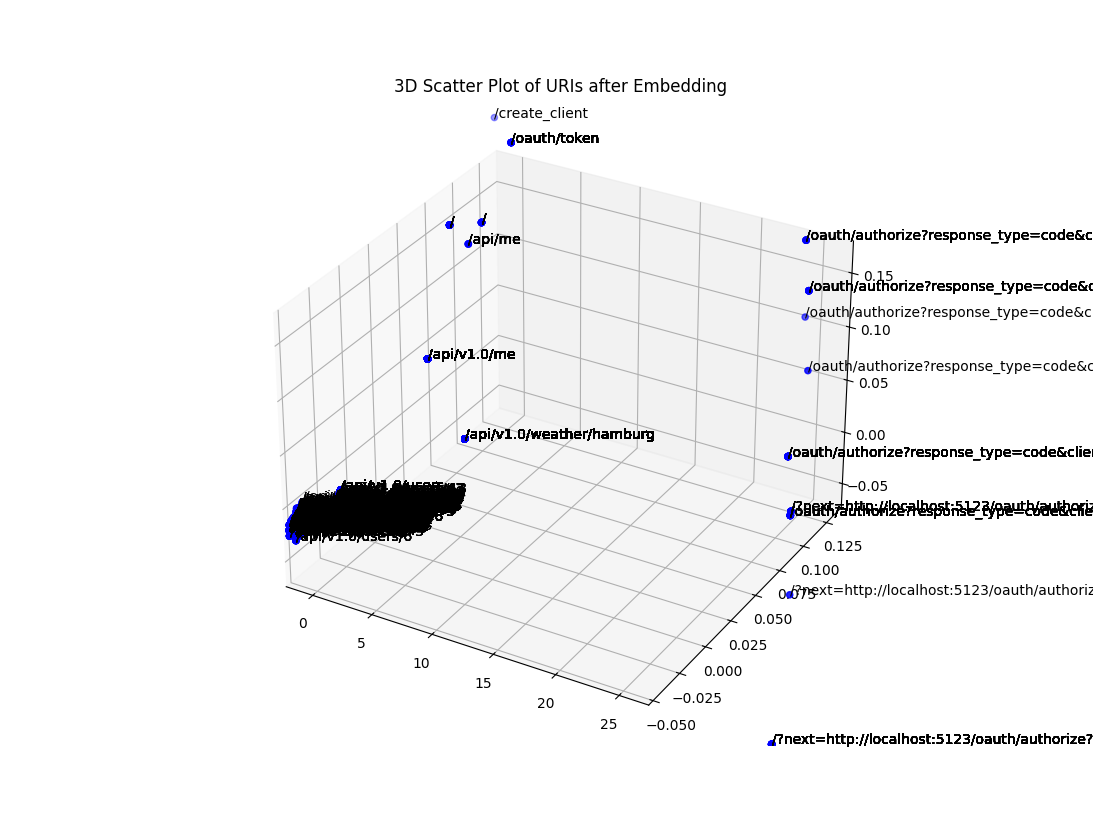
\includegraphics[width=1\textwidth]{pic/word_embeddings_3d.png}
	\unitlength=0.75mm
	\special{em:linewidth 0.4pt}
	\linethickness{0.4pt}
	\caption{Embedding Vectors normalized to three dimensions. Every point in the plot represents one record of the dataset. The word2vec embedding approach leads to a clear group and some sets of outliers.}
	\label{fig:word_embeddings3D}
\end{figure}

\subsection{Overall anomaly detection results}
The overall results after clustering are showcased in Table \ref{tab:results}. Both clustering algorithms achieve the same results with a high accuracy of >99\% but, in relation, only attain a low precision score after the word2vec embedding. The main observation which leads to these results is that the implemented approaches perform well in filtering out traffic not involved in OAuth but do not achieve the same quality of detection in more subtle differences in the OAuth traffic itself. Also, achieving the same results for both clustering algorithms could mean that the main impact for anomaly detection in this scenario lies in the encoding step with word2vec. These observations are discussed further in Section \ref{subsec:results_discussion} after the following sections explain how the clustering algorithms achieve their results.

\begin{table}[H]
	\caption{Results of Intrusion Detection using Word2Vec and Clustering algorithms}
	\label{tab:results}
	\begin{tabular}{|l|l|l|}
	\hline
					   & \textbf{k-means} & \textbf{Self-Organizing Maps} \\ \hline
	\textbf{Accuracy}  & 0.993            & 0.993                         \\ \hline
	\textbf{Yield}     & 1.0              & 1.0                           \\ \hline
	\textbf{Precision} & 0.637            & 0.637                         \\ \hline
	\end{tabular}
\end{table}

\subsubsection{Anomaly detection with k-means}
\label{subsubsec:anom_k_means}
The first observation on the k-means clustering results is the behaviour when setting different cluster sizes for the algorithm for an anomaly threshold of 5\%. The results show that after slowly increasing the number of clusters k-means calculates, a decay of accuracy and precision appears after 7 clusters as depicted in Table \ref{tab:k-means_clusters}. The reason is that k-means starts to split larger groups of records into clusters small enough to be detected as anomalous at some point and many of these larger groups are non-attack traffic. As depicted in Figure \ref{fig:kmeans_clusters_2}, when only two clusters are calculated, a large group of non-attack traffic records exist near the origin, and some smaller outlier groups, including attack traffic, appear further away from the origin. Figure \ref{fig:kmeans_clusters_6} shows that k-means starts to split the large cluster of non-attack traffic near the origin into smaller clusters when the cluster number is set to 6. Experimenting with the threshold on a higher number of clusters also leads to the highest achievable precision of 0,637\%, for example, when setting the number of clusters to 24 and the threshold to 0,39\%.

\begin{table}[H]
	\caption{Setting a higher number of k-means clusters to calculate leads to decay in accuracy and precision starting at 8 clusters with an anomaly threshold of 5\%}
	\label{tab:k-means_clusters}
	\begin{tabular}{|l|c|c|c|c|c|c|c|c|c|c|}
	\hline
	\textbf{k-means Clusters}   & \textbf{2} & \textbf{3} & \textbf{4} & \textbf{5} & \textbf{6} & \textbf{7} & \textbf{8} & \textbf{17} & \textbf{20} & \textbf{24} \\ \hline
	\textbf{Anomalous Clusters} & 1          & 2          & 2          & 2          & 3          & 4          & 5          & 10          & 12          & 18          \\ \hline
	\textbf{Accuracy}           & 0,99       & 0,99       & 0,99       & 0,99       & 0,99       & 0,99       & 0,97       & 0,92        & 0,89        & 0.71        \\ \hline
	\textbf{Precision}          & 0,63       & 0,63       & 0,63       & 0,63       & 0,63       & 0,63       & 0,34       & 0,13        & 0,11        & 0,05        \\ \hline
	\end{tabular}
\end{table}

\begin{figure}[H]
	\caption{Word2Vec and k-means setting 2 clusters}
	\label{fig:kmeans_clusters_2}
	\sffamily\footnotesize
	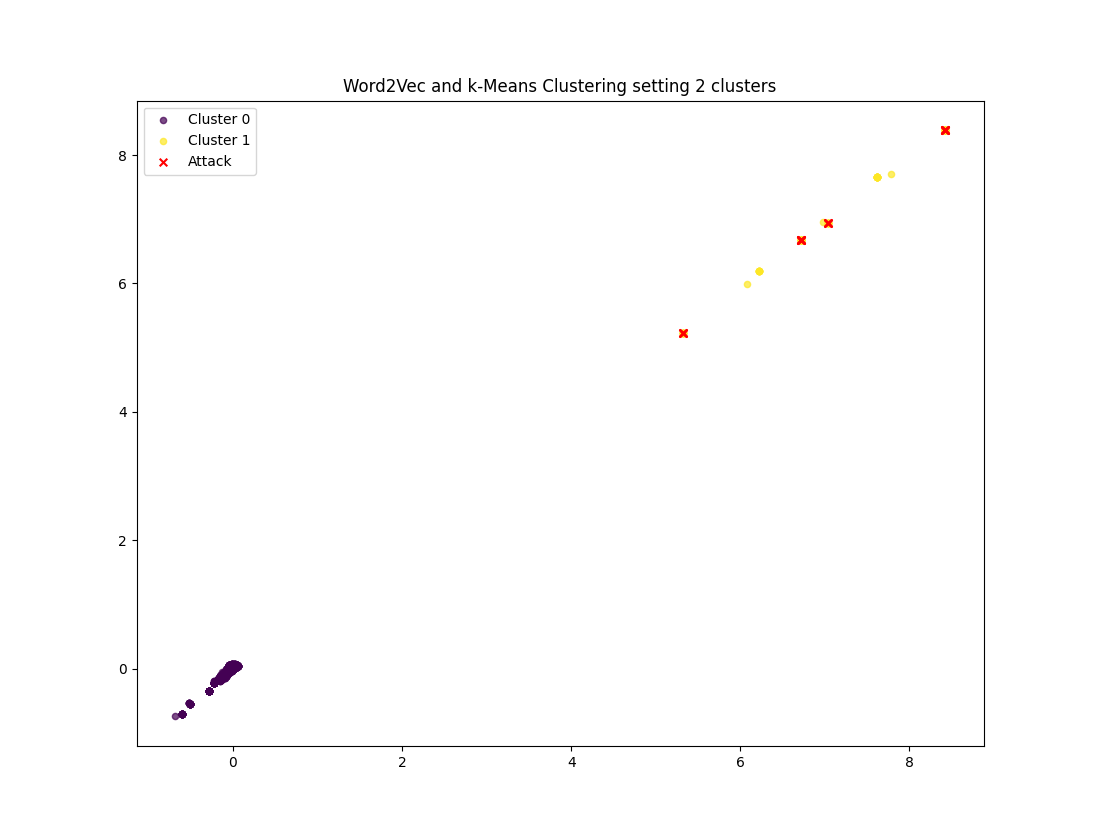
\includegraphics[width=1\textwidth]{pic/k_means_2.png}
	\unitlength=0.75mm
	\special{em:linewidth 0.4pt}
	\linethickness{0.4pt}
\end{figure}

\begin{figure}[H]
	\caption{Word2Vec and k-means setting 6 clusters}
	\label{fig:kmeans_clusters_6}
	\sffamily\footnotesize
	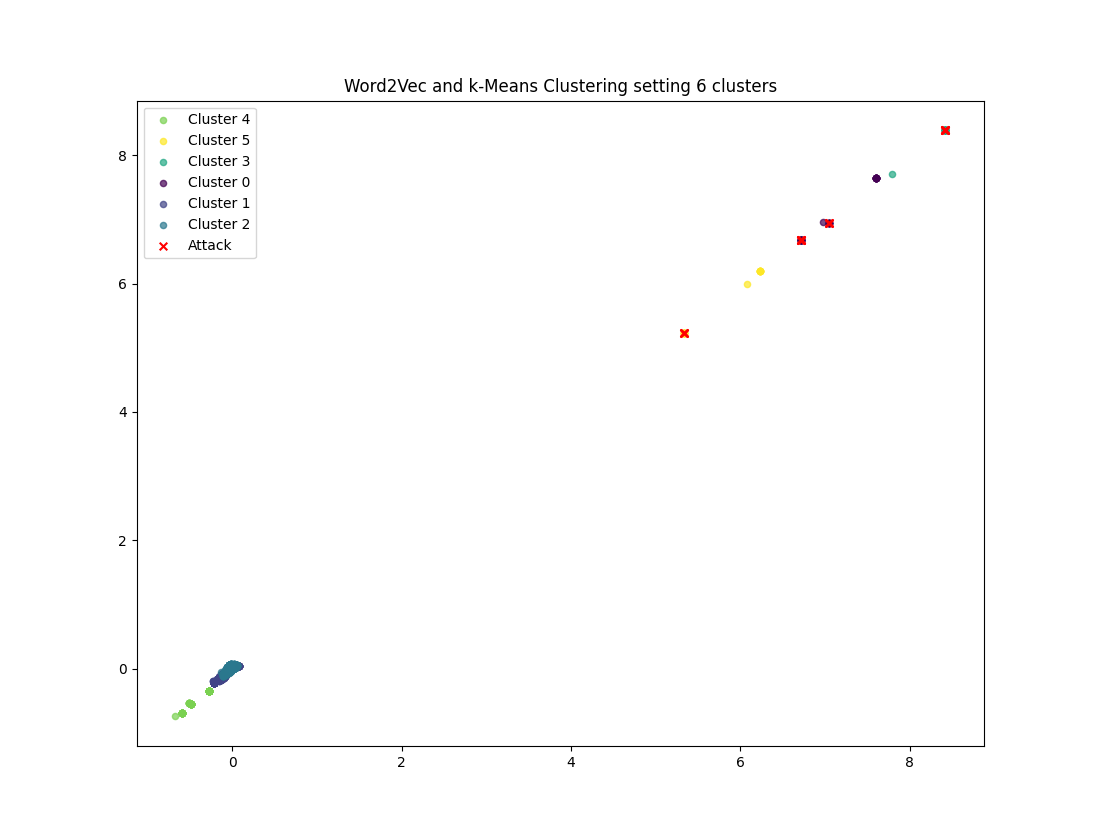
\includegraphics[width=1\textwidth]{pic/k_means_6.png}
	\unitlength=0.75mm
	\special{em:linewidth 0.4pt}
	\linethickness{0.4pt}
\end{figure}

\subsubsection{Anomaly detection with self-organizing maps}
The self-organizing maps clustering approach leads to the same results as the k-means clustering algorithm. Figure \ref{fig:som_clusters} shows that the algorithm creates three clusters, one of which is an attack cluster. In the figure, it is also visible that SOM is splitting the main group of records near the origin, a non-attack traffic group, into two clusters that are large enough to be considered non-anomalous. Tuning the hyperparameters only leads to the result that fewer iterations of training are needed to achieve the same best accuracy and precision. 



\begin{figure}[H]
	\caption{Word2Vec and Self-Organizing Maps}
	\label{fig:som_clusters}
	\sffamily\footnotesize
	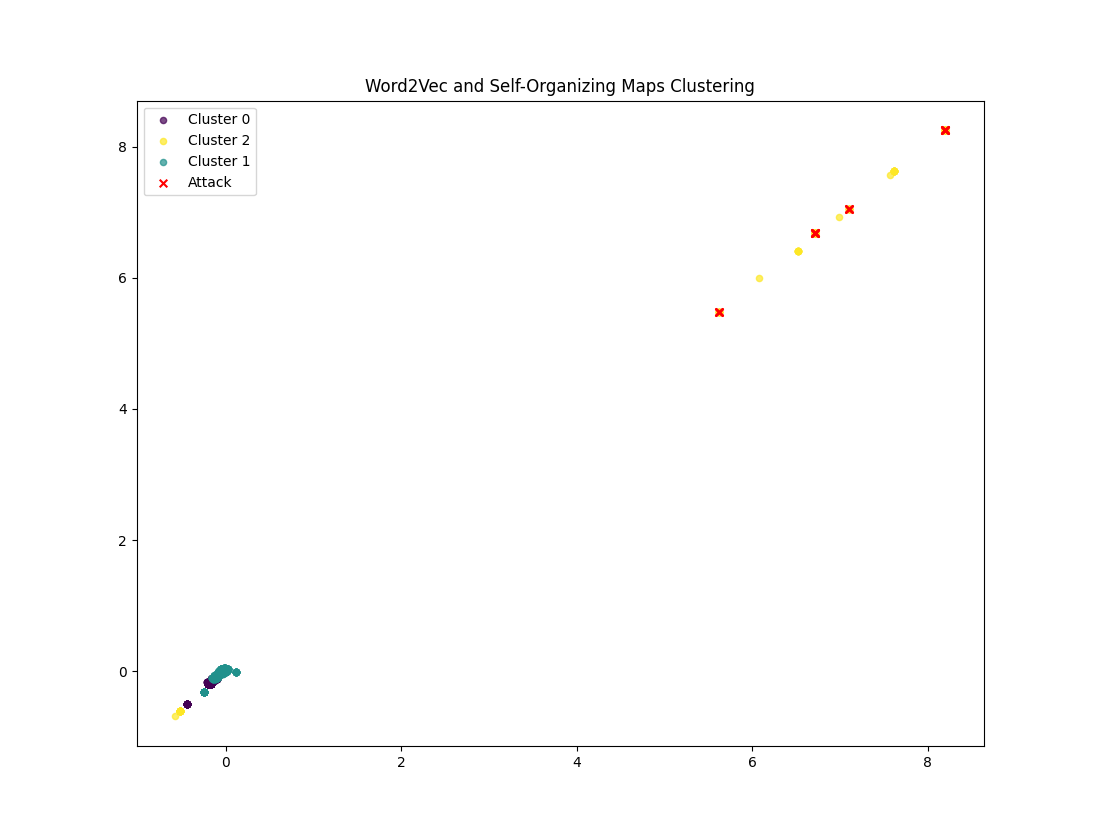
\includegraphics[width=1\textwidth]{pic/som_final.png}
	\unitlength=0.75mm
	\special{em:linewidth 0.4pt}
	\linethickness{0.4pt}
\end{figure}


\subsection{Discussion of methodology and results}
\label{subsec:results_discussion}

The results clearly show that the embedding approach greatly impacts the results in the given scenario. The scenario itself, however, is artificial and created through simulating traffic. This approach is arguably too sparse, but a dataset containing specific attacks on the OAuth protocol was not available at the time of this writing. Hence, this model for intrusion detection was created for this work. The dataset simulates real-world HTTP packet data using valid implementations of the OAuth protocol. It does not model metadata of the network traffic, as it does not model real-world timings and flow data of different actors and attackers accessing a network. Consequently, this research focuses on analyzing the semantics of the involved HTTP application data instead of the states and transitions of the protocol flow. 

The attack type integrated into the dataset was chosen because attacks on OAuth manipulating the redirect flow are highly impactful concerning the takeover of accounts and extracting confidential data. Attacks involving multiple auth providers, like Mix-Up attacks, were not included as detecting these kinds of attacks would require sophisticated data about the timings and transitions of the network data, which is not provided by the modelled dataset and could only realistically be provided by a real-world network, which was not available for the scope of this work.

The encoding of the application data, based on previous research by Corizzo et al. \cite{corizzo2020feature}, is a highly promising approach for extracting features for network data, which is why it was applied in this work. However, the low diversity of attacks outside the OAuth traffic influences the performance of this approach in this modeled data. Other classifier methods were tested to achieve anomaly detection before choosing the clustering approach for this work. Supervised learning classifiers like support vector machines were tested but not further researched as the narrow model of network data quickly led to overfitting and a classifier that would have a 100\% precision rate only inside the modeled data. Consequently, researching clustering methods with word embeddings was the most promising approach to detecting anomalies, meaning detecting even unknown attacks outside the modeled dataset.

As protocols for the internet like OAuth 2.0 grow in complexity over time, the approach of detecting anomalies in the application data of the protocol gains importance as well since some types of attacks exploit subtle logical implementation flaws, like the redirect manipulation attacks implemented in this work. Therefore, this research bears relevance for future methods in detecting anomalies in application data, even though the dataset is artificially generated.